\documentclass[11pt]{article}

\usepackage[a4paper, margin=1in]{geometry}
\usepackage{graphicx}
\usepackage{hyperref}
\usepackage{xcolor}
\usepackage{titlesec}
\usepackage{colortbl}
\usepackage{tikz}
\usetikzlibrary{positioning, shapes.geometric, arrows.meta, backgrounds}

\definecolor{cmuRed}{HTML}{C41230}
\definecolor{lightGray}{HTML}{F1F3F5}

\hypersetup{
    colorlinks=true,
    linkcolor=black,
    urlcolor=cmuRed
}

\titleformat{\section}{\Large\bfseries\color{cmuRed}}{}{0em}{}[\vspace{0.2em}\titlerule]

\begin{document}

\begin{center}
\vspace*{-0.8cm}
{\Huge\bfseries\textcolor{cmuRed}{CountsFor}}\\[0.1cm]
{\large 3-Week Redesign Plan: Visual Summary}\\[0.1cm]
{\scriptsize Prepared by Aditya Vivek \& Hind Jendara}
\end{center}
\vspace{-0.4cm}
\rule{\textwidth}{0.4pt}
\vspace{-0.4cm}


\section*{Welcome \& Concept}
\vspace{-0.3cm}
Welcome to the \textbf{CountsFor} project proposal! This guide explains what we're building over the next 3 weeks. We're replacing the current clunky interface with a modern foundation that uses "live" data.

\vspace{0.1cm}
\noindent \textbf{The Data Flow:}
\vspace{0.1cm}
\begin{center}
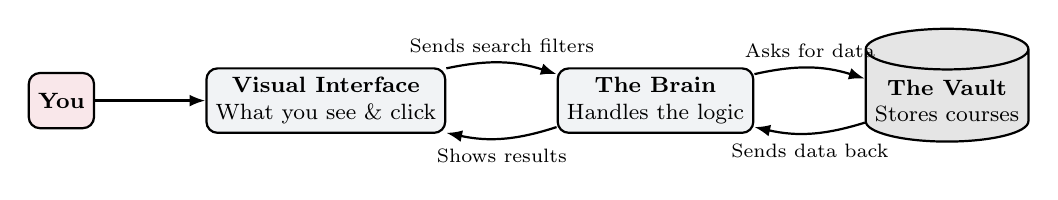
\begin{tikzpicture}[
    node distance=1.1cm and 1.4cm,
    font=\footnotesize,
    box/.style={rectangle, draw, rounded corners, minimum height=0.7cm, align=center, fill=lightGray, thick},
    arrow/.style={-{Latex[length=2mm]}, thick}
]

\node[box, fill=cmuRed!10] (user) {\textbf{You}};
\node[box, right=of user] (ui) {\textbf{Visual Interface}\\What you see \& click};
\node[box, right=of ui] (brain) {\textbf{The Brain}\\Handles the logic};
\node[cylinder, draw, shape border rotate=90, aspect=0.25, thick, fill=gray!20, right=of brain, align=center] (vault) {\textbf{The Vault}\\Stores courses};

\draw[arrow] (user) -- (ui);
\draw[arrow] (ui) edge[bend left=15] node[above, font=\scriptsize] {Sends search filters} (brain);
\draw[arrow] (brain) edge[bend left=15] node[below, font=\scriptsize] {Shows results} (ui);

\draw[arrow] (brain) edge[bend left=15] node[above, font=\scriptsize] {Asks for data} (vault);=
\draw[arrow] (vault) edge[bend left=15] node[below, font=\scriptsize] {Sends data back} (brain);

\end{tikzpicture}
\end{center}
\vspace{-0.2cm}

\noindent \textbf{1. Visual Interface:} What you see and click.\\
\textbf{2. The Brain:} Handles the middle-man logic and sorting.\\
\textbf{3. The Vault:} Where all course data is securely stored.

\section{Proposed Visuals}
\vspace{-0.2cm}
We are revamping the look to be minimal, responsive, and easy on the eyes. 

\subsection*{The Main Course Catalog}
Below is a concept wireframe of what the main Search/Catalog page will look like. Notice the clean top bar, the organized filters, and the easily readable table.

\begin{figure}[h]
\centering
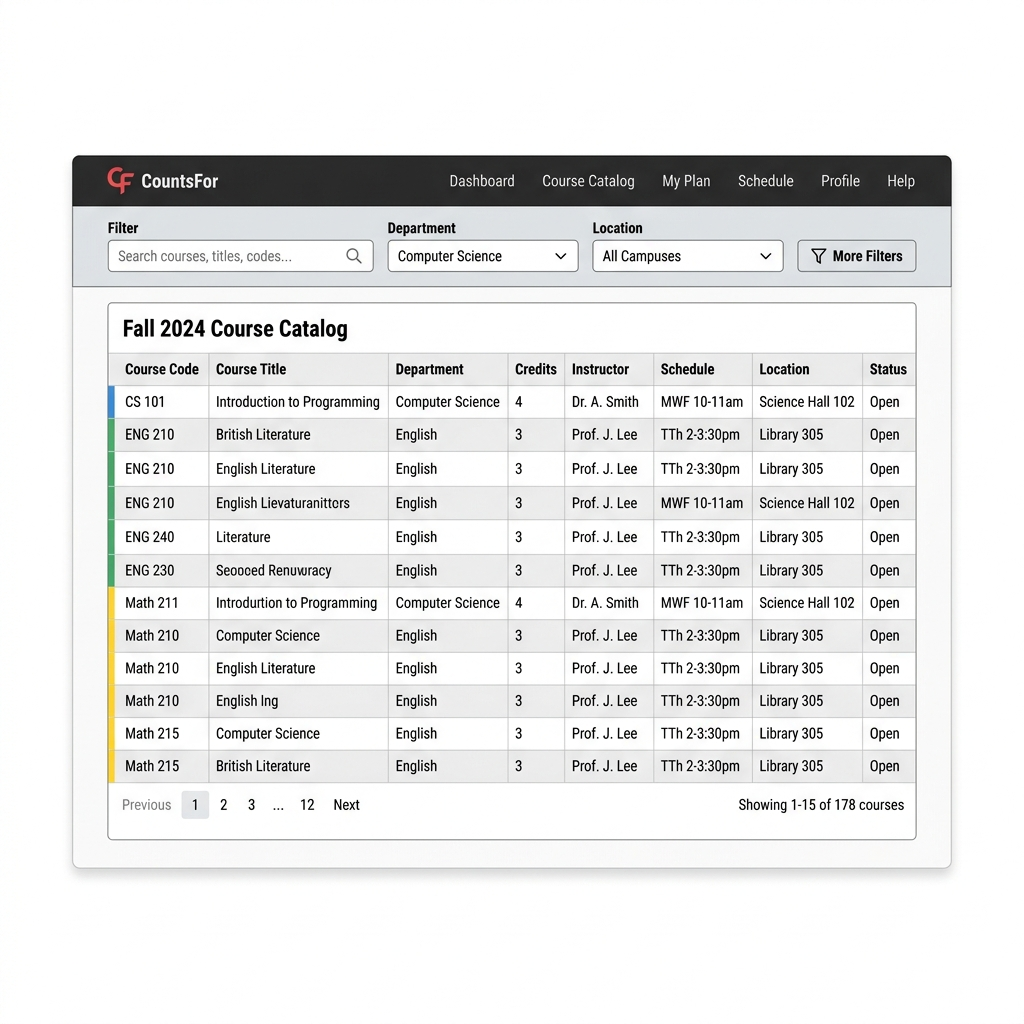
\includegraphics[width=0.85\textwidth]{countsfor_wireframe_main.png}\\[0.2cm]
\textit{\small Note: This is just a rough conceptual wireframe to give a general idea. The final design will be much more refined and detailed.}
\end{figure}

\textbf{Key Improvements Here:}
\begin{itemize}
    \item \textbf{Slim Top Bar}: Taking up way less space so you can actually focus on the courses.
    \item \textbf{Unified Filters}: Simple dropdowns for Department, Location, and Course Type all in one row.
    \item \textbf{Muted Colors}: Using softer colors for the different majors so it's not blindingly bright.
\item \textbf{Working Sort}: Click headers to sort rows.
\end{itemize}

\vspace{-0.2cm}
\subsection*{The 'My Plan' Tab}
\vspace{-0.2cm}
Select courses and save them for advising meetings.

\begin{figure}[h]
\centering
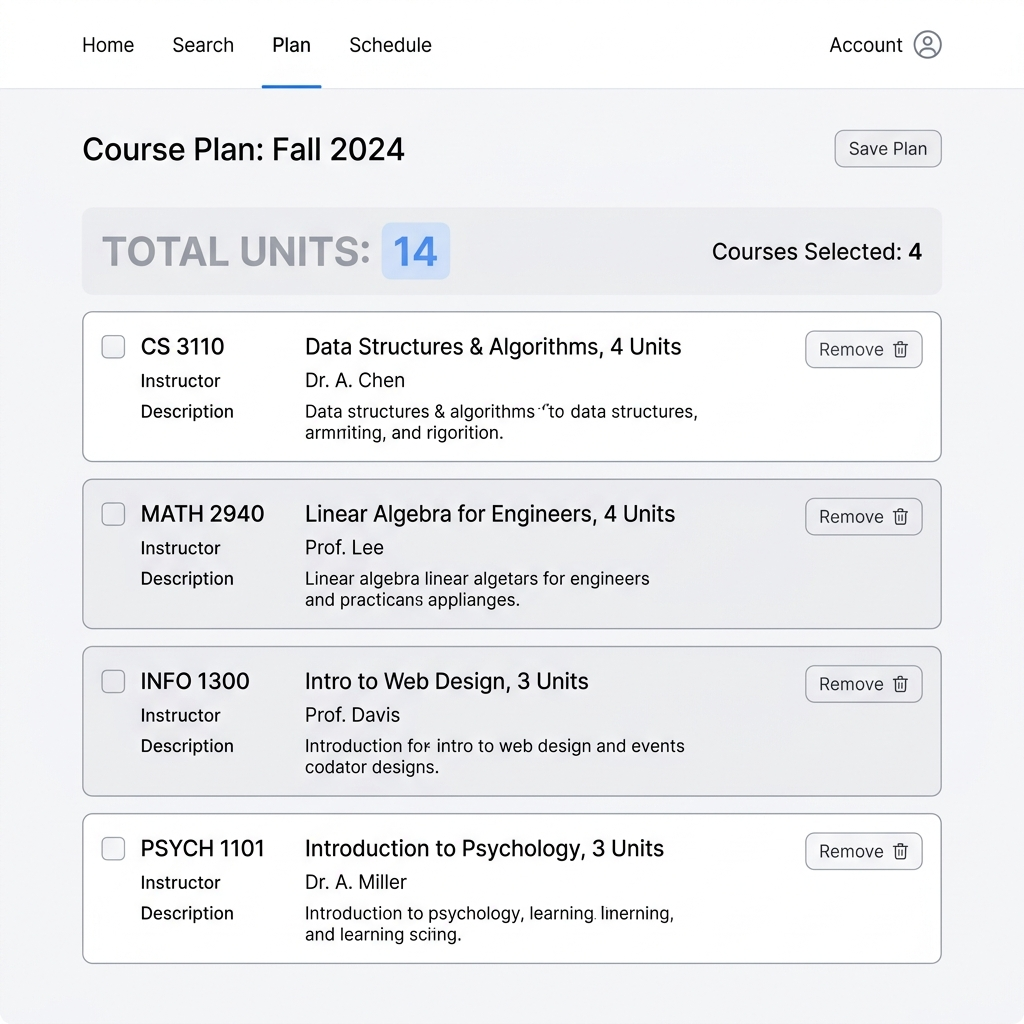
\includegraphics[width=0.7\textwidth]{countsfor_wireframe_plan.png}\\[0.2cm]
\textit{\small Note: This is just a rough conceptual wireframe to give a general idea. The final design will be much more refined and detailed.}
\end{figure}

\textbf{Key Improvements Here:}
\begin{itemize}
    \item \textbf{Running Total}: Easily see how many units you are currently "registered" for.
    \item \textbf{Clean List}: A straightforward list of what you've picked.
    \item \textbf{Auto-Save}: If you refresh the page or close your laptop, your plan will still be there when you come back.
\end{itemize}

\section{Our 3-Week Timeline}
\vspace{-0.3cm}
\begin{center}
\renewcommand{\arraystretch}{1.1}
\small
\begin{tabular}{|p{0.3\textwidth}|p{0.3\textwidth}|p{0.3\textwidth}|}
\hline
\rowcolor{cmuRed!10}
\textbf{Week 1 (Apr 5-11)} & \textbf{Week 2 (Apr 12-18)} & \textbf{Week 3 (Apr 19-23)} \\
\hline
\textbf{Aditya (Visual)} \newline Layout, colors, & 
\textbf{Aditya (Visual)} \newline Table styling, & 
\textbf{Aditya \& Hind} \newline Testing, polish, \\
\& project shell. & dark mode. & debugging. \\
\hline
\textbf{Hind (Backend)} \newline Database setup & 
\textbf{Hind (Backend)} \newline Connecting UI & 
\textbf{Phase 1 Complete} \newline Plan \& Foundation \\
\& migration. & to data/API. & done by Apr 23. \\
\hline
\end{tabular}
\end{center}

\vspace{-0.2cm}
\section{Deferred to Summer}
\vspace{-0.3cm}
The following items are out of scope for the current 3-week sprint:
\begin{itemize}[noitemsep, nolistsep]
    \item \textbf{Mobile Layout}: Guaranteed not to break, but not optimized for small screens yet. 
    \item \textbf{Animations \& Analytics}: Transitions and dashboards will be built later.
    \item \textbf{Auto-updates}: Course data is currently a snapshot; auto-syncing comes in Summer.
\end{itemize}

\vspace{0.5cm}
\begin{center}
\rule{0.5\textwidth}{0.4pt} \\
\textit{\small Prepared for the Management Team}
\end{center}

\end{document}
